\begin{frame}{Previous/\alert{Our} Work (non exhaustive)}
    \begin{figure}
    \centering
    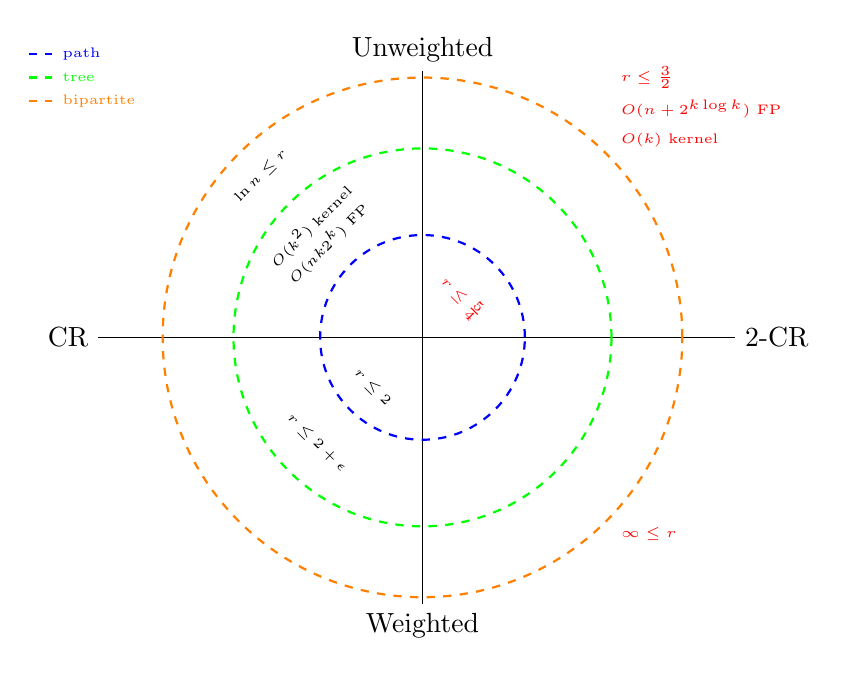
\begin{tikzpicture}[every node/.style={draw=none}]
    
    \node(cr) at(-4.5,0) {CR};
    \node(2cr) at(4.5,0) {2-CR};
    
    \node(weighted) at(0,-3.66) {Weighted};
    \node(unweighted) at(0,3.66) {Unweighted};
    
    \draw[] (cr) -- (2cr);
    \draw[] (weighted) -- (unweighted);
    
    \begin{scope}[thick, dashed]
    
    \draw[blue]	(-5,3.6) -- +(0.3,0) node[right]{\tiny path};
    \draw[green]	(-5,3.3) -- +(0.3,0) node[right]{\tiny tree};
    \draw[orange]	(-5,3) -- +(0.3,0) node[right]{\tiny bipartite};
    
    \draw[blue] (0,0) circle(1.3cm);
    \draw[green] (0,0) circle(2.4cm);
    \draw[orange] (0,0) circle(3.3cm);
    \end{scope}
    
    \begin{scope}[every node/.style={rotate=-45}]
    \node at(225:.9){\tiny$r \leq 2$};
    \node at(225:1.9){\tiny$r \leq 2 + \epsilon$};
    \end{scope}
    
    \begin{scope}[every node/.style={rotate=45}]
    \node at(135:1.7){\tiny $O(n k 2^{k})$ FP};
    \node at(135:2){\tiny $O(k^2)$ kernel};
    \node at(135:2.9){\tiny$\ln n \leq r$};
    \end{scope}
    
    \node[red, rotate=-45] at(45:.7){\tiny $r \leq \frac{5}{4}$};
    \begin{scope}[anchor=west]
    \node[red] at(2.4,2.5){\tiny $O(k)$ kernel};
    \node[red] at(2.4,2.9){\tiny $O(n + 2^{k\log k})$ FP};
    \node[red] at(2.4,3.3){\tiny $r \leq \frac{3}{2}$};
    \node[red] at(2.4,-2.5){\tiny $\infty \leq r$};
    \end{scope}
    
    \begin{scope}[]
    \end{scope}
    
    \end{tikzpicture}
    \end{figure}
    \end{frame}